% The random states one compiled function draws from, and their views:
% the arguments are flattened into leaves, a random state contributing two (its
% key and its counter), and each random state among the arguments has a view
% of its own, identified by the AnvlTracedRandomState the function receives for
% it; the global random state is taken
% as implicit inputs. After the run,
% on_success() finds each argument's random state again by that leaf and
% advances it by the draws the trace counted for it.
% Build: see figures/README.md
\documentclass[tikz, border = 6pt]{standalone}
\usepackage[T1]{fontenc}
\usepackage{lmodern}
\usepackage{amsmath}
\usetikzlibrary{positioning, calc, arrows.meta, fit, backgrounds}

\definecolor{hash}{HTML}{5B8C5A}
\definecolor{keep}{HTML}{2A7AB0}
\definecolor{fork}{HTML}{E08A2C}

\tikzset{
  >={Stealth[length = 2mm]},
  coltitle/.style = {font = \small\bfseries, text = black!70},
  arg/.style = {draw = black!50, fill = white, rounded corners = 2pt,
    inner sep = 3pt, font = \ttfamily\footnotesize, minimum height = 5.5mm},
  rngnode/.style = {draw = fork!80!black, fill = fork!15, rounded corners = 2pt,
    inner sep = 3pt, font = \ttfamily\footnotesize, minimum height = 5.5mm},
  leaf/.style = {draw = black!50, fill = white, inner sep = 2.5pt,
    font = \ttfamily\footnotesize, minimum height = 5.5mm, minimum width = 3.3cm,
    anchor = west},
  rngleaf/.style = {leaf, draw = fork!80!black, fill = fork!10},
  inst/.style = {draw = hash!80!black, fill = hash!15, rounded corners = 2pt,
    inner sep = 4pt, font = \footnotesize, align = left, anchor = west},
  globinst/.style = {inst, draw = keep!80!black, fill = keep!15},
  num/.style = {font = \footnotesize, text = black!55, anchor = east},
  note/.style = {font = \footnotesize, text = black!65, align = left},
  edge/.style = {->, black!60},
  tree/.style = {black!45}
}

\begin{document}
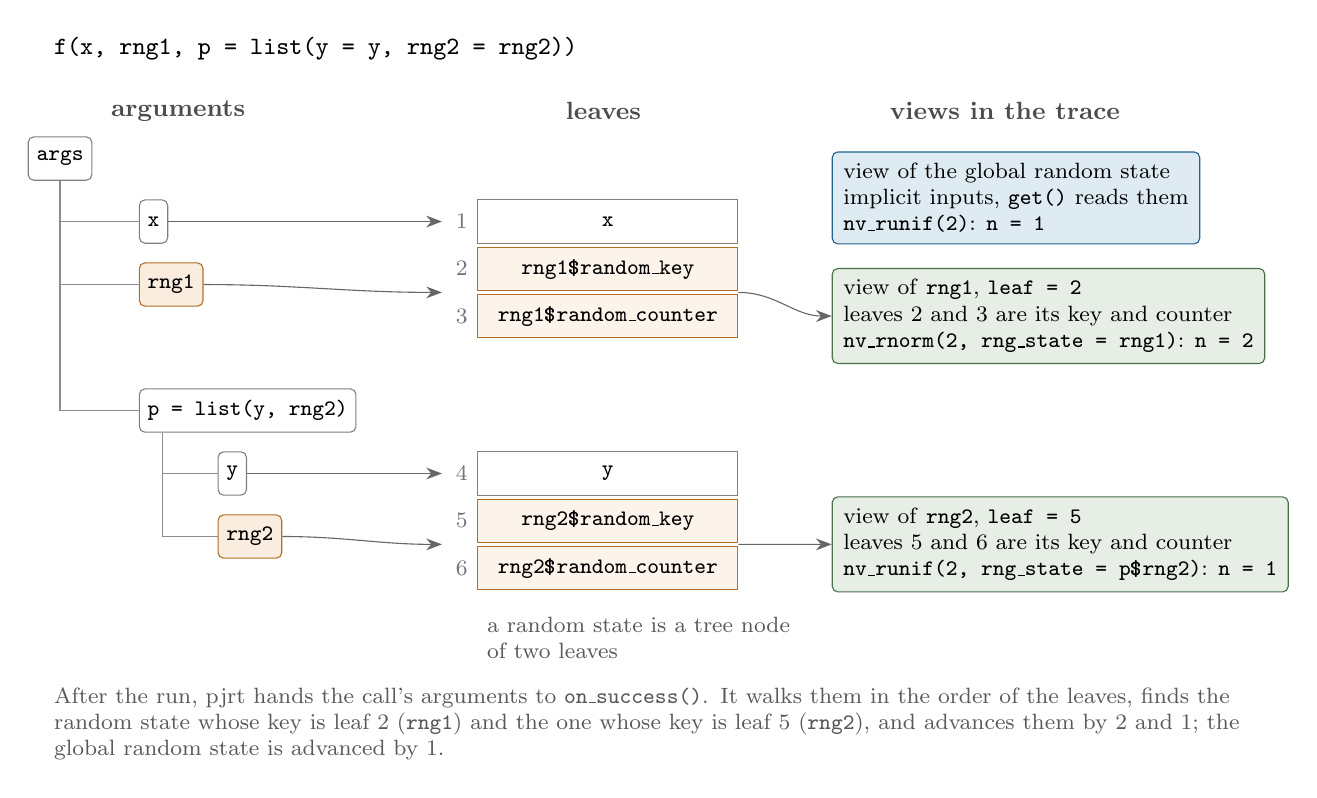
\begin{tikzpicture}

  % ---- the call ------------------------------------------------------------
  \node[font = \ttfamily\small, anchor = west] at (-0.2, 1.4)
    {f(x, rng1, p = list(y = y, rng2 = rng2))};

  % ---- the arguments as a tree ---------------------------------------------
  \node[coltitle] at (1.5, 0.6) {arguments};
  \node[arg] (root) at (0.0, 0) {args};
  \node[arg, anchor = west] (x) at (1.0, -0.8) {x};
  \node[rngnode, anchor = west] (r1) at (1.0, -1.6) {rng1};
  \node[arg, anchor = west] (l) at (1.0, -3.2) {p = list(y, rng2)};
  \node[arg, anchor = west] (y) at (2.0, -4.0) {y};
  \node[rngnode, anchor = west] (r2) at (2.0, -4.8) {rng2};
  \foreach \n in {x, r1, l} \draw[tree] (root.south) |- (\n.west);
  \foreach \n in {y, r2} \draw[tree] ($(l.south west) + (0.3, 0)$) |- (\n.west);

  % ---- the leaves ----------------------------------------------------------
  \node[coltitle] at (6.9, 0.6) {leaves};
  \node[leaf]    (L1) at (5.3, -0.8) {x};
  \node[rngleaf] (L2) at (5.3, -1.4) {rng1\$random\_key};
  \node[rngleaf] (L3) at (5.3, -2.0) {rng1\$random\_counter};
  \node[leaf]    (L4) at (5.3, -4.0) {y};
  \node[rngleaf] (L5) at (5.3, -4.6) {rng2\$random\_key};
  \node[rngleaf] (L6) at (5.3, -5.2) {rng2\$random\_counter};
  \foreach \i in {1, ..., 6} \node[num] at (L\i.west) {\i\ };
  \draw[edge] (x.east) -- ($(L1.west) + (-0.45, 0)$);
  \draw[edge] (r1.east) to[out = 0, in = 180] ($(L2.west)!0.5!(L3.west) + (-0.45, 0)$);
  \draw[edge] (y.east) -- ($(L4.west) + (-0.45, 0)$);
  \draw[edge] (r2.east) to[out = 0, in = 180] ($(L5.west)!0.5!(L6.west) + (-0.45, 0)$);
  \node[note, anchor = north west] at (5.3, -5.7)
    {a random state is a tree node\\of two leaves};

  % ---- the views in the trace ----------------------------------------------
  \node[coltitle] at (12.0, 0.6) {views in the trace};
  \node[globinst] (G) at (9.8, -0.5)
    {view of the global random state\\
     implicit inputs, \texttt{get()} reads them\\
     \texttt{nv\_runif(2)}: \texttt{n = 1}};
  \node[inst] (I2) at (9.8, -2.0)
    {view of \texttt{rng1}, \texttt{leaf = 2}\\
     leaves 2 and 3 are its key and counter\\
     \texttt{nv\_rnorm(2, rng\_state = rng1)}: \texttt{n = 2}};
  \node[inst] (I5) at (9.8, -4.9)
    {view of \texttt{rng2}, \texttt{leaf = 5}\\
     leaves 5 and 6 are its key and counter\\
     \texttt{nv\_runif(2, rng\_state = p\$rng2)}: \texttt{n = 1}};
  \draw[edge] ($(L2.east)!0.5!(L3.east)$) to[out = 0, in = 180] (I2.west);
  \draw[edge] ($(L5.east)!0.5!(L6.east)$) to[out = 0, in = 180] (I5.west);

  % ---- after the run -------------------------------------------------------
  \node[note, anchor = north west, text width = 15.2cm] at (-0.2, -6.6)
    {After the run, pjrt hands the call's arguments to \texttt{on\_success()}.
     It walks them in the order of the leaves, finds the random state whose key
     is leaf 2 (\texttt{rng1}) and the one whose key is leaf 5 (\texttt{rng2}),
     and advances them by 2 and 1; the global random state is advanced by 1.};

\end{tikzpicture}
\end{document}
